% !TEX root = ../thesis.tex
\chapter{Simulating Cyber-Physical Systems in the Virtual-World (10)}
% Describe what better CPS tools would provide - environmental simulation, trained environment models, virtual environments, cross-environment simulation

Testing and understanding how the environment interacts with a sensor network and vice-versa relies on placing the devices in the target environment and waiting for/creating the desired phenomena to interact with the network. Performing tests in the real-world is time-consuming, costly and often impractical. Carrying out tests utilising human mobility also poses difficulties. Phenomena can include events such as movement of devices/objects, passive or active interaction with people (pressing buttons, triggering motion sensors), or other sensor events. Performing test deployments can be expensive, time-consuming and difficult.


% In this chapter we present and evaluate a novel approach to this problem, integrating a freely available high-performance 3D video game engine (Unreal Engine 4) with an existing sensor network simulation platform (Cooja), creating an end-to-end simulation solution for realistic testing of sensor networks in their target environments. By integrating a 3D game engine, we are introducing sensor network simulations into virtual reality with a real-time and dynamic virtual world, utilising the game engine's realistic physics, lighting and artificially intelligent people and crowds to influence and test the deployed sensor network.

% In the following section we describe in detail our novel 3D simulation platform, Ard\'{a}n, discussing the various features and tools it provides. Section 2 discusses the requirements which we believe to be vital for 3D simulation platform development. Section 3 describes the design and architecture of Ard\'{a}n, followed by an example case study for testing and deployment in section 4. We subsequently present a performance evaluation and discuss the challenges involved in developing the Ard\'{a}n platform, in sections 5 and 6 respectively.
\section{Problem} % (fold)
\label{sec:problem}
Cyber-physical systems are deployed in physical environments, interacting with the surrounding physical infrastructure to provide services for nearby inhabitants, such as heating, lighting, security, fire and environmental safety. However, existing simulation tools and techniques used to develop, test and analyse such systems don't consider the physical environment, its inhabitants and their mobility. 
 
Existing approaches for testing CPS focus heavily on accurately simulating devices, the network and power consumption, with great success \cite{cooja, tossim}. These tools and techniques don't support reliably, comprehensively and dynamically testing these devices in the context of their target environment and the phenomena which may occur within it. 

\subsection{Simulation Issues} % (fold)
\label{ssub:simulation_issues}

% subsubsection simulation_issues (end)
Typically, the environment data is fed into simulations using recorded sensor data (traces) from an existing deployment or field study\cite{bridge,Gaglione2018}, or is fabricated based on a developer's conceptual model and testing needs. These traces suffer from several issues:
\begin{itemize}
  \item \textbf{Acquisition} - traces need to be recorded from existing real-world deployments or field studies, the former may not match the target network, and the later can be time-consuming, expensive, dangerous, or inconvenient to perform thoroughly.
  \item \textbf{Static} - recorded traces are taken from fixed positions, and can't be modified after-the-fact.
  \item \textbf{Reliability} - fabricated traces are based on a developers model of an environment and may not accurately represent it or all of it.
  \item \textbf{Comprehensive} - traces are time consuming to create and must be created ahead of time, thus, limiting the number of traces created.
  \item \textbf{Scalability} - updating or modifying traces to support new devices being added or when the scenario changes becomes unmanageable for even small networks.
\end{itemize}

\subsection{Deployment and Test-bed Issues} % (fold)
\label{ssub:deployment_and_test_bed_issues}

% subsubsection deployment_and_test_bed_issues (end)
For CPS involving human and device mobility, deployment and test-beds\cite{wisebed1,wisebed2,TempLab,dependibilityTestbedChallenge} are not only time-consuming and expensive to deploy, but also are limited by health and safety, people recruitment, location availability, and scalability issues.

\begin{itemize}
  \item \textbf{Health and Safety} - Testing involving people needs to ensure strict health and safety guidelines and laws are adhered to, requiring participants to be safeguarded against possible injury and death, thus, testing situations in which poses a threat to participants can't be carried out. 

  \item \textbf{Recruitment} - Recruiting participants also makes real-world testing difficult, as tests may require large numbers of people and relatively mundane activities. 

  \item \textbf{Location availability} - Exclusive access to target locations prior to full deployment for testing can be difficult at peak times, requiring out-of-hours testing on weekends or evenings. This can have a knock on impact for recruiting participants.

  \item \textbf{Scalability} - Running tests with extremely large numbers of people at once e.g., >50 for an evacuation, requires significant planning and management. Similarly, running large numbers of tests with even a small number of people may simply not be possible due to time constraints, thus, only a core set of tests may be carried out instead, limiting the scope.

  \item \textbf{Realism} - It's not possible to run tests with real people in real evacuation scenarios, due to health and safety. Instead we can simulate these scenarios in the real-world using fire-drills; however, fire drills by nature have an impact on how people may act during an evacuation. Similarly, people may become familiar with the environment the more tests they perform, which could affect their reaction time and the choices they make. 
\end{itemize}


In the rest of this chapter, we introduce a novel CPS co-simulation platform that has been developed to tackle the issue of simulating a CPS with realistic, dynamic and flexible environment input, described above; the design of the co-simulation platform is based on the framework described in chapter \ref{chap:framework}.


% section problem (end)
\section{A 3D Virtual World Co-Simulation Platform} % (fold)
\label{sec:a_3d_co_simulation_platform}

To meet the needs of testing CPS with realistic, dynamic and flexible environment input we designed and built an open co-simulation platform that integrates WSN simulation with a 3D game engine. 

\subsection{The 3D Game Engine Component} % (fold)
\label{sub:a_3d_game_engine}

% subsection a_3d_game_engine (end)
Using the 3D game engine, we're able to create vivid and realistic models of the real world, involving complex physics, AI pedestrians and crowds, physical destruction, and lighting. In games, films and TV these effects are used purely for creating immersive experiences which can trick the viewer into suspending disbelief; within a simulation these can be instead used effectively to create living simulations grounded in reality. 

Using these features, we can:
\begin{itemize}
   \item \textbf{Physics} - simulate CPS which involve movement and actuation which are affected by the laws of the physical world, including gravity, friction and momentum, enabling dynamic and flexible simulations.
   \item \textbf{AI pedestrians and crowds} - simulate human-centric CPS such as in offices, schools or stadiums, with pedestrians and crowds exhibiting desired behaviours, such as goal-based movement, avoidance, herding, panic, etc.
   \item \textbf{Physical Destruction} - simulate destructible environments and buildings, which can dynamically react to virtual earthquakes, explosions or other destructive phenomena.
   \item \textbf{Lighting} - simulate realistic lighting effects, such as shadows, fire and smoke, allowing viewers to understand how lighting and visibility may be affected by different sources of light (sun, lamps, lights, fire) and in different scenarios, day-to-day office, fire evacuation etc. 
 \end{itemize} 


 Using the input from the 3D game engine to drive the CPS simulation which can then drive change in the virtual world, creates truly dynamic and reactive closed-loop simulations; such a system removes the need for developers to gather, fabricate, modify or update individual sensor traces. This gives developers more time to focus on building better CPS based on their tests, than building the tests.

 We believe utilising a 3D game engine to drive the CPS simulation can help resolve the simulation issues described previously, section \ref{ssub:simulation_issues}:
 \begin{itemize}
  \item \textbf{Acquisition} - developers can model 3D environments which match the design, layout and conditions of their target environment.
  \item \textbf{Dynamic and Reactive} - new traces are generated in real-time based on the CPS and environment as it changes, be it a new layout or pedestrian behaviour reacting to the CPS or other phenomena.
  \item \textbf{Reliable} - the game engine simulates a virtual world grounded by realistic physics and lighting. Therefore, relieving the burden on the programmer of creating realistic input models, e.g., calculating when a person will intercept motion sensors as they walk down a corridor. AI people and crowds can be programmed based on desired needs e.g., herding, follow, avoid behaviours.
  \item \textbf{Comprehensive} - simulations can be carried out faster than real-time, combined with the dynamic physics-based world enables many different scenarios to be tested out in significantly less time.
  \item \textbf{Scalable} - as new devices are added or existing ones moved, the simulation dynamically adapts and creates a new trace.
\end{itemize}

Similarly, we believe this co-simulation approach can begin to address the deployment and test-bed issues described in section \ref{ssub:deployment_and_test_bed_issues}.

\begin{itemize}
  \item \textbf{Health and Safety} - Virtual tests involve virtual people, hence, health and safety rules need not apply. However, one envisions they could apply to some extent if real people are used for virtual reality (VR) tests, but with much less risk attached e.g., real people can't be physically burned by a virtual fire, although they may experience VR sickness.

  \item \textbf{Recruitment} - Participant recruitment is a non-issue, within a 3D game engine world, 100's of AI participants can be created as and when needed, no bribing necessary.

  \item \textbf{Location availability} - Locations can be modelled in the 3D world based off a floor-plan, requiring no access to the real physical location. Alternatively, a one-time measurement plan can be carried out with minimal interference caused.

  \item \textbf{Scalability} - It is possible to run tests with large numbers of people 24/7, without issue or complaints, scheduling issues or location availability issues.

  \item \textbf{Realism} - AI people and crowds can mimic required behaviour, enabling perhaps more consistent simulations when compared to real people in fake or ``drill'' scenarios, e.g., virtual people can be told to panic or mimic herding behaviour, whereas real people may not exhibit this behaviour in non-life-threatening scenarios. This enables developers to test for these different behaviours and scenarios which affect them. However, the AI behaviour may not reflect the true unique and complex reactions of a real person and crowd in real scenarios.
\end{itemize}

\subsection{The WSN/CPS Simulator Component} % (fold)
\label{sub:a_wsn_cps_simulator}
Like previous physical simulator approaches \cite{6815220}, we could use a standard programming language and environment to program and model the WSN component, such as the language used within the game engine, C++. However, this approach has several limitations:
\begin{itemize}
  \item \textbf{Portability} - programming in a non-WSN/CPS language and environment requires porting to the desired platform when deploying. This can vary in difficulty depending on the differences in language, environment and programming paradigm/model e.g., event-based or imperative.
  \item \textbf{Accuracy} - many issues in WSN/CPS depend on the performance constraints of the deployment devices which have severely limited CPU, RAM, ROM and battery hardware.
  \item \textbf{Radio Network} - WSN/CPS rely on their radio network for communicating between nodes within a network, which also has a significant impact on other aspects of the device, such as performance, duty cycle and battery life.
\end{itemize}

Utilising the Cooja WSN simulator enables the co-simulation platform to build upon the tool to create a powerful testing platform which developers can test on before seamlessly deploying to real devices in their target environment.

\begin{itemize}
  \item \textbf{Portable} - Cooja nodes are programmed in the Contiki C language, hence, the same code can be deployed for simulated nodes as for deployed nodes. This removes the issues related to translating between simulated and real nodes.
  \item \textbf{Accurate} - Cooja nodes can be simulated at various accuracy levels, using the same code, dependent on the level needed and the available computing power of the host simulation PC.
  \item \textbf{Radio Simulation} - Cooja provides various radio simulation models, enabling developers to test complex radio scenarios, with varying RSSI and interference models. 
\end{itemize}
% subsection a_wsn_cps_simulator (end)
% section a_3d_co_simulation_platform (end)

\section{Co-Simulator Design}
\label{sec:Design}
Discussed in chapter \ref{chap:framework}, the co-simulation platform is designed in an open, component agnostic fashion, i.e., the platform encourages the interoperability of different simulation platforms, specifying clear abstractions and boundaries between components. The goal is to create a plug-n-play platform that can support the use of different simulation, analytical and game engine tools, with our implementation providing an example construction.

\subsection{WSN Simulator Component} % (fold)
\label{sub:wsn_simulator_component}

The WSN simulator, Cooja, performs the hardware, software and radio network simulation for each node within a WSN in the co-simulation. 
Users select the hardware they wish to deploy there application code, software, to, which is then compiled for the desired platform. Depending on the level of accuracy, host PC performance and size of the desired network, developers can select the hardware simulation level they wish the node to be simulated at, which ultimately dictates whether the code is compiled to the target or host architecture. This enables developers to sacrifice hardware accuracy for a larger simulated network.

\subsubsection{Radio} % (fold)
\label{ssub:radio}

Radio simulation is performed entirely within Cooja, relying on the built-in radio models and distance between nodes to determine node RSSI and packet-loss. \textbf{Utilising the game engine's knowledge of the 3D world and obstructions between nodes could improve the accuracy of the radio simulation, however, this remains as future work. Kokkinis et al.\cite{trunetWireless} have demonstrated the use of 3D models of target environments to simulate an accurate radio model based on obstructions and their material types.}


% subsubsection radio (end)
\subsubsection{Location} % (fold)
\label{ssub:location}

Each node is configured with an initial 3D location, used in the radio simulation to calculate radio interference. The location is exposed to other co-simulation components via pub/sub topics which Cooja is subscribed to, so can be updated at any time by other co-simulation components (game engine), creating dynamic mobile nodes which can then affect Cooja's radio simulation.
% subsubsection location (end)

\subsubsection{Hardware Interfaces - Sensors} % (fold)
\label{ssub:hardware_interfaces_sensors}

Hardware interfaces which normally interact with the physical world, such as motion/acceleration/light sensors or buttons, are exposed as virtual hardware interfaces to other co-simulation components via pub/sub topics.

\missingfigure{Will show how - Node hardware interfaces connect to other components via a publish/subscribe bus.}

Data related to input interfaces can be published to by co-simulation components, to which Cooja subscribes and distributes to the relevant nodes, such that when a node queries a sensor, the most up-to-date reading is available. This also ensures response time for hardware interface requests is kept to the absolute minimal.

Similarly, data related to output interfaces, such as LEDs or actuators, is published by Cooja to the relevant per-interface topics; allowing subscribed components to be updated in real-time of hardware events, which can then be actioned in a virtual world component, recorded by a logging or analytical component.


% subsubsection hardware_interfaces_sensors (end)
% subsection wsn_simulator_component (end)

\subsection{3D Game Engine Component} % (fold)
\label{sub:3d_game_engine_component}
The 3D game engine component, Unreal Engine 4, is responsible for simulating the 3D virtual world and the physics, lighting and people within it. It also models the physical manifestation of the nodes and their exposed hardware interfaces, such as sensors and lights.

\subsubsection{Virtual Node Hardware} % (fold)
\label{ssub:virtual_node_hardware}
Within the virtual world we can choose to model node hardware to an accurate scale, or not. This allows for developers to choose physical accuracy when required for scenarios which may involve mobile nodes which can be affected by physics and collisions with the environment. On the other hand, increasing a nodes scale can help locatability of a node and visibility of any information on the device, such as LEDs or an ID.

\begin{figure}[h]
   \centering
   \includegraphics[width=\textwidth]{img/sensorScales.png}
   \caption{Variable sensor scales, providing either physically accurate sized devices or more visible devices}
   \label{fig:sensor_scales}
 \end{figure} 
% subsubsection virtual_node_hardware (end)
Within the game engine we can model the target 3D environment and created a several components to support deploying virtual sensor networks, including device and sensor 3D models, hardware abstractions for the virtual sensors and actuators to sense the virtual world and report back to the simulator over the network bus. Similarly within the Cooja simulator we have modified the simulated hardware to communicate to our virtual hardware in the Unreal Engine.
\subsubsection{Virtual Environment} % (fold)
\label{ssub:virtual_environment}

% subsubsection virtual_environment (end)

\subsubsection{AI People and Crowds} % (fold)
\label{ssub:ai_people_and_crowds}

% subsubsection ai_people_and_crowds (end)
Using Cooja, developers are able to write code once and both test in Ard\'{a}n and deploy in the real-world on the Contiki or TinyOS platform, removing difficulties associated with translating between test and deployment platforms. Using the open architecture, support for additional tools and simulation platforms can also be added, expanding the possibilities and improving the fidelity of simulations.

% subsection 3d_game_engine_component (end)
\section{Phenomena-on-demand} % (fold)
\label{sec:phenomena_on_demand}
Unlike existing approaches which utilise purely trace-fed and scripted approaches which are static and difficult to modify, this simulator enables dynamic phenomena generation based on the user input or scripted behaviour. 
By taking direct control of devices or people within the environment, developers can interact with and modify the simulation directly and observe how the dynamic simulation responds. This differs to trace-fed alternatives which require developers to manually change the input to sensors based on how they believe the environment has changed. 

For example, two sensors are placed within a school corridor to detect the pace of people walking past; the sensors communicate and calculate the walker's pace, displaying a red light to people running. In a trace-fed scenario, developers script sensor detection inputs to the two nodes. Developers may generate a test case for different speed walkers or multiple walkers. For each test case, the developers need to manually calculate and modify each trace-feed for each sensor individually. For our approach, developers need only change the speed of a person walking and observe the effects on the system. This approach provides a much more intuitive and scalable solution to testing with large numbers of devices and as the number of input sensors increase, in which trace-fed solutions become unmaintainable.  
% section phenomena_on_demand (end)

\section{Mobility} % (fold)
\label{sec:mobility}

% section mobility (end)
\section{Communication} % (fold)
\label{sec:communication}

% section communication (end)
\section{Synchronisation} % (fold)
\label{sec:synchronisation}

% section synchronisation (end)



\section{Forward Time Control} % (fold)
\label{sec:time_control}

\section{Distribution} % (fold)
\label{sec:distribution}

% section distribution (end)

\section{Case Study}
\label{sec:Case Study: Corridor}

The purpose of the following case study is to demonstrate what development of a non-trivial CPS application is like using Ard\'{a}n, and how it enables developers to test and visualise different scenarios, by simply adding or moving devices or people in the simulation.

The case study focuses on controlling the lighting within a modern day office corridor, with the goal of striking a balance between energy efficiency, effective lighting and user comfort. The ideal corridor lighting scheme should provide a pleasant lighting scheme for users of the corridor, able to adjust based on ambient light levels, gradually illuminating as they progress through it, whilst also ensuring energy is minimised by turning off or reducing the brightness of unused or infrequently used parts of the corridor.

Thus, this provides an interesting and non-trivial task, due to the many ways in which the corridor can be entered/exited or moved around within in; people can enter from the beginning, end or from a room; people can move down the length of the corridor or directly from room to room; people often also stop in the corridor, spending time talking or waiting. Similarly, understanding the ideal number and placement for devices and sensors, and how it affects applications, such as power, reliability, robustness etc. Hence, providing effective lighting schemes can prove difficult to analyse and reason without rigorous testing.

The rest of this section will demonstrate and discuss the use of Ard\'{a}n to design, analyse and test for our target environment, the corridor, highlighting the features and benefits that the tool provides.


\begin{figure*}[t]
  \centering
  \subfloat[Over-the-shoulder view]{
    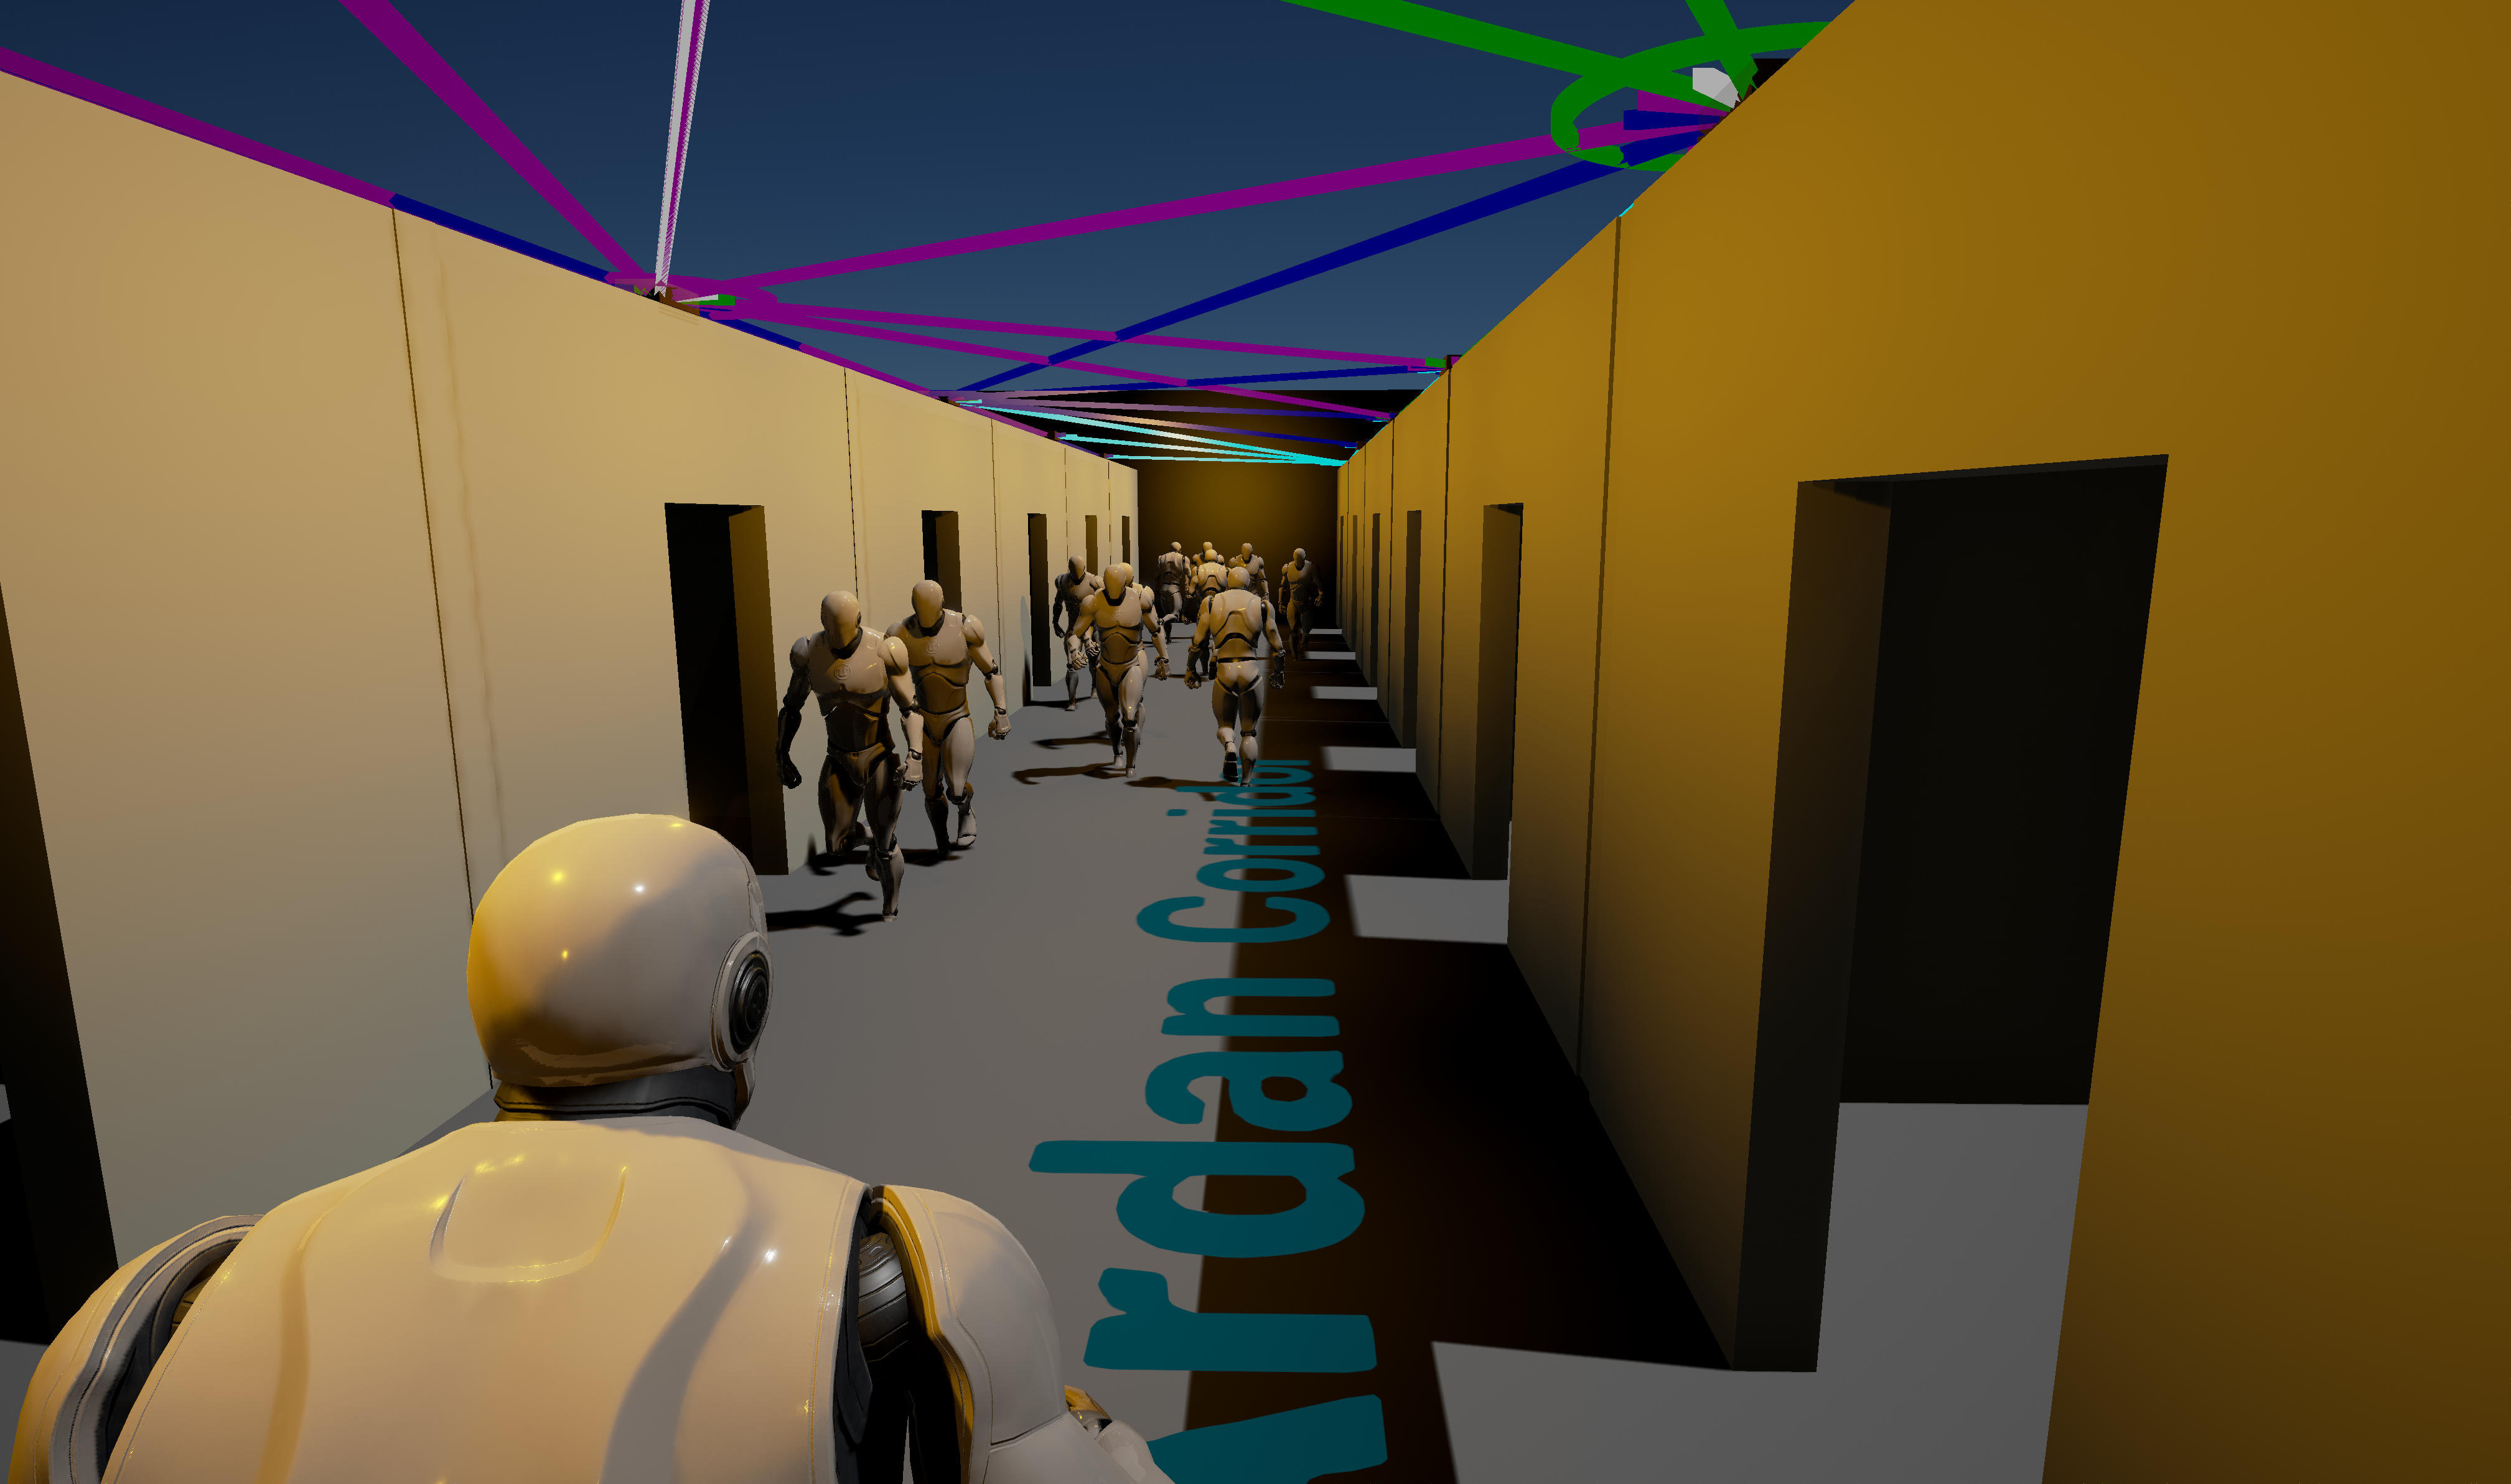
\includegraphics[height=2.6cm]{imgs/OverShoulder.jpg}
    \label{fig:birds_view}
  }
  \subfloat[Birds-eye view]{
    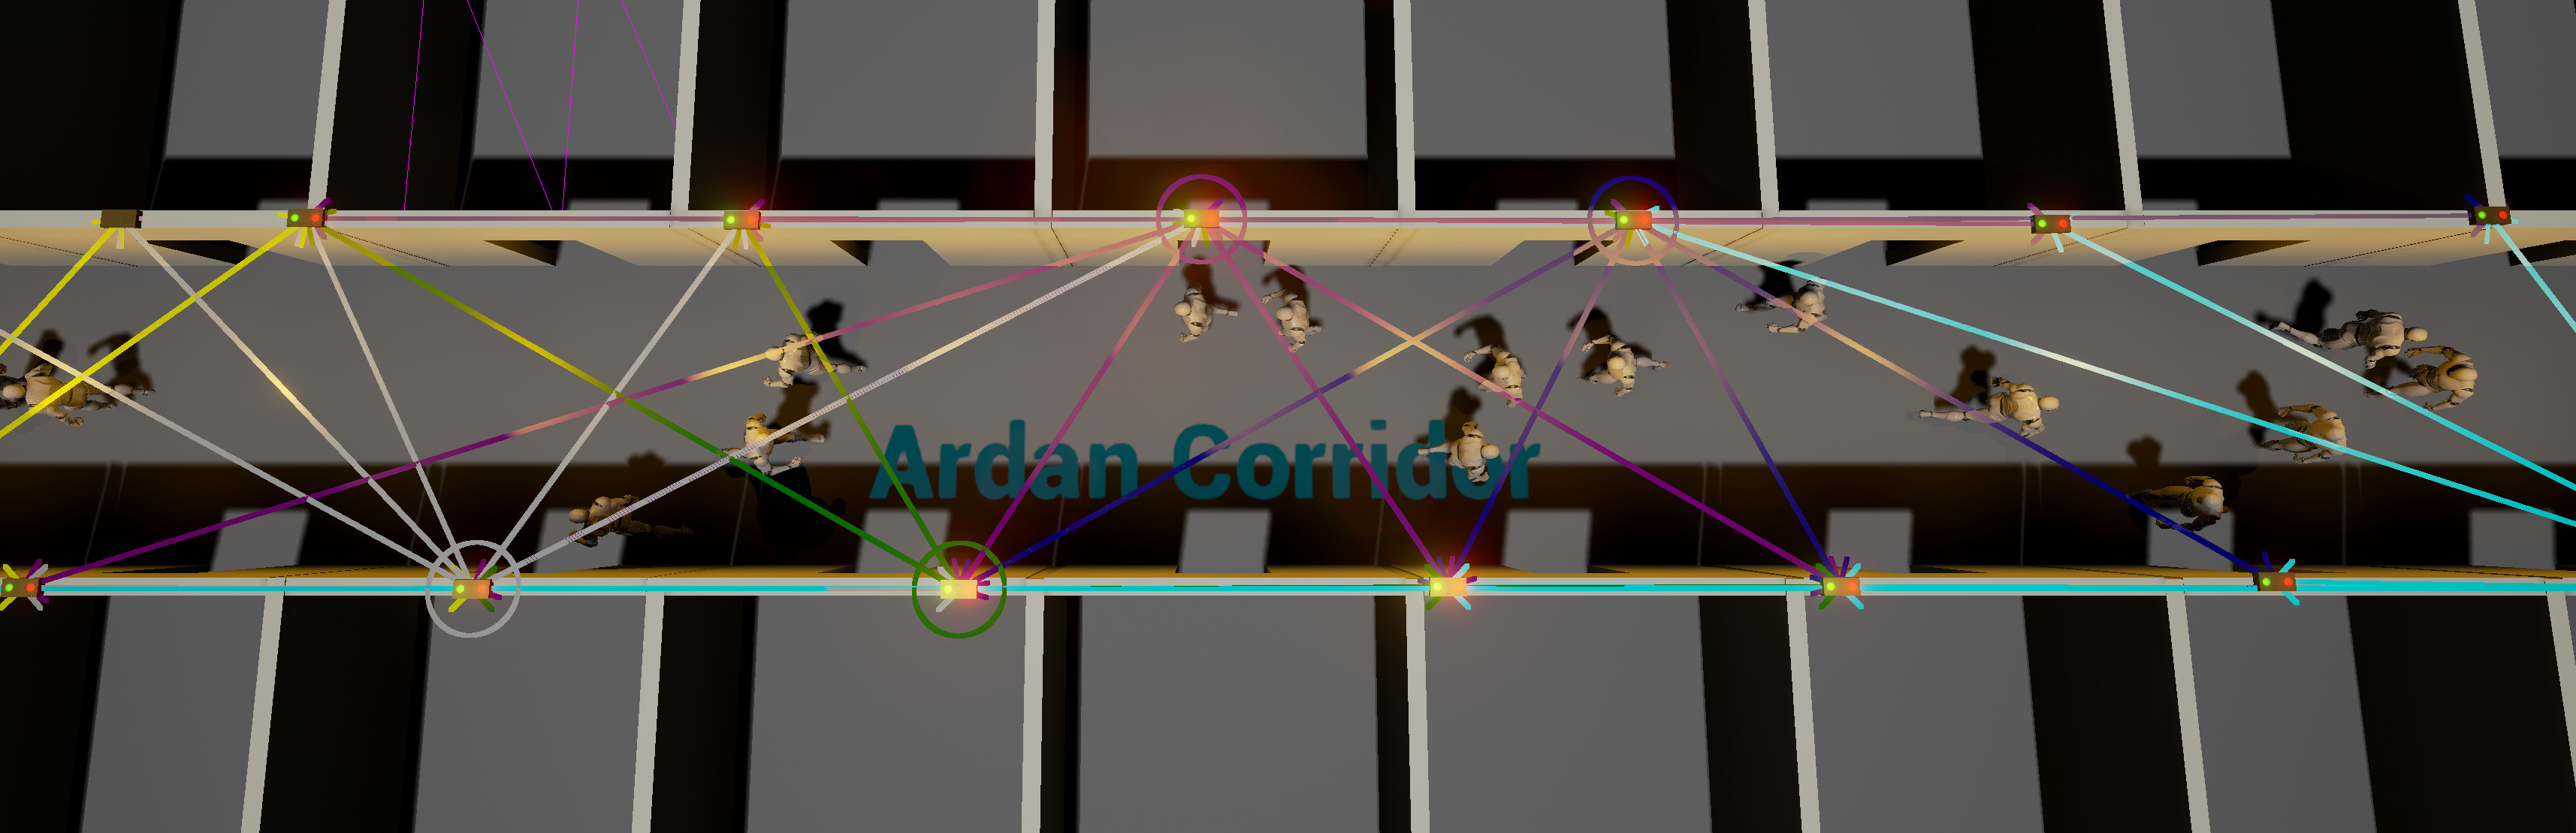
\includegraphics[height=2.6cm]{imgs/BirdsEye2.jpg}
    \label{fig:shoulder_view}
  }
  \subfloat[Camera view]{
    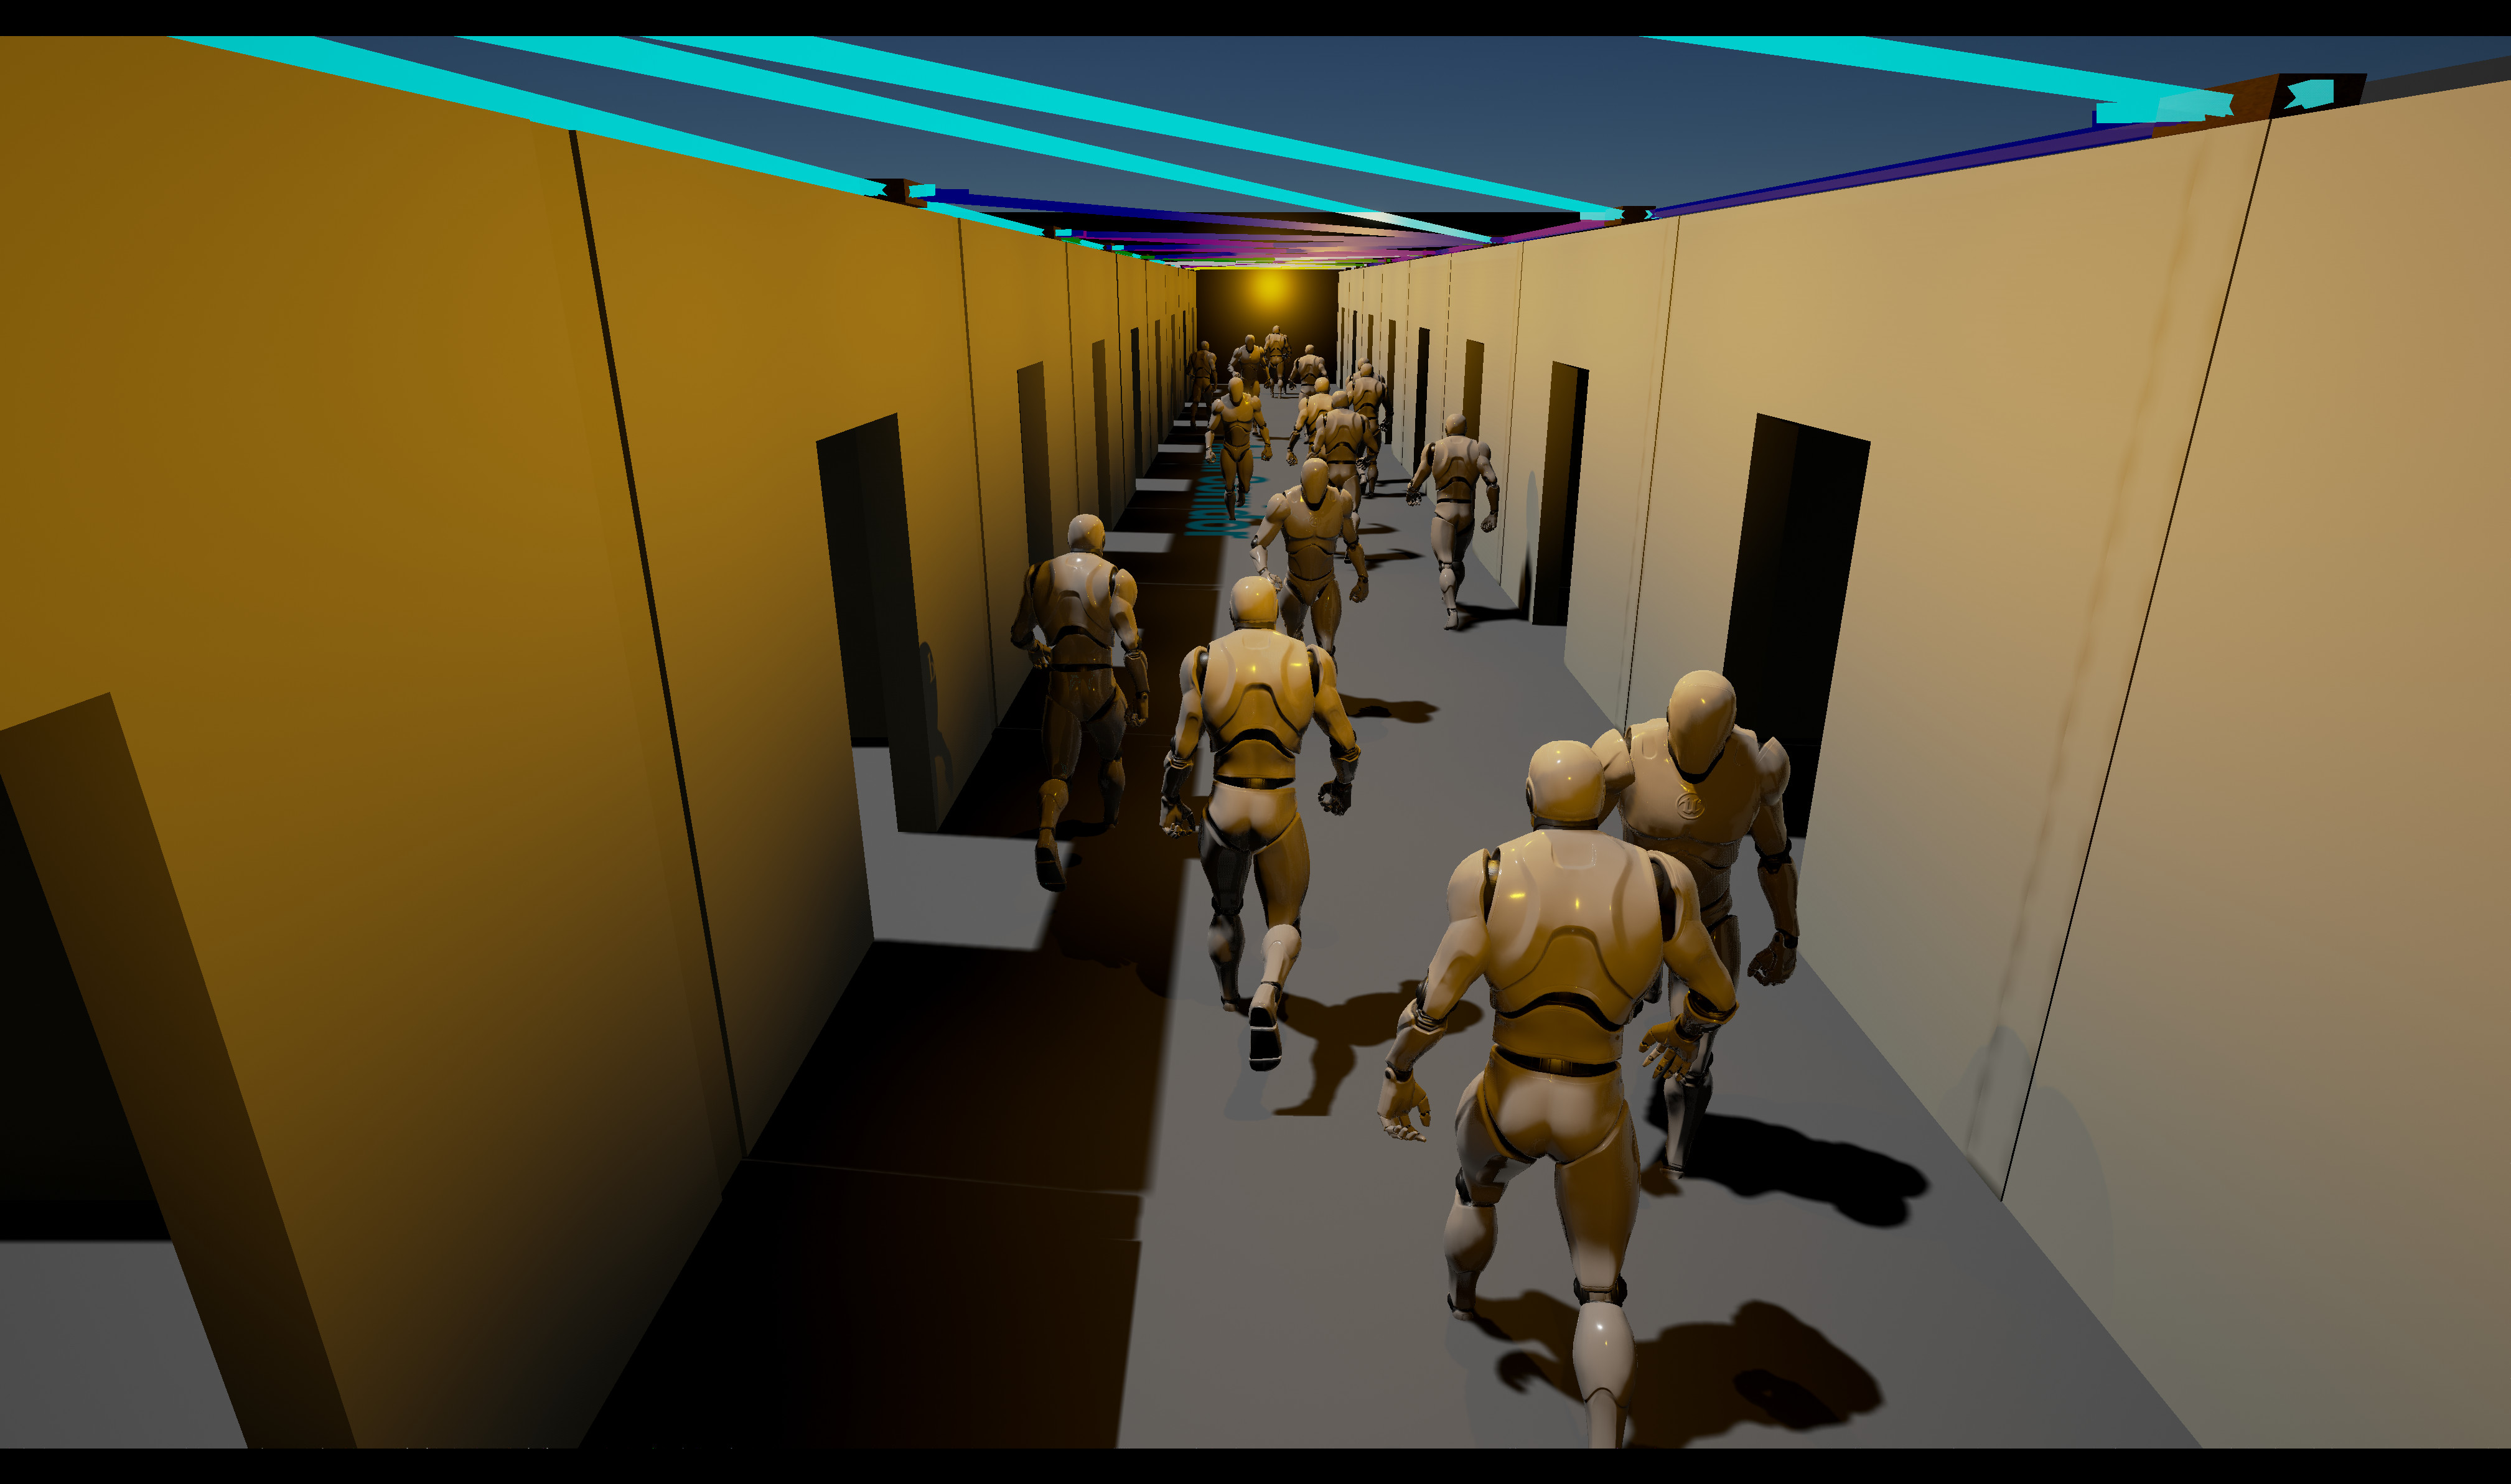
\includegraphics[height=2.6cm]{imgs/Camera.jpg}
    \label{fig:camera1_view}
  }
  \caption{15 people walking up and down the virtual corridor, triggering motion sensors}
  \label{fig:views}
\end{figure*}


\subsection{Corridor Design}
\label{sub:Constructing the corridor}
We created a virtual corridor based on a real corridor within our building, measuring 20x 1.5 meters, with 5 doors spaced evenly on either side. Along the corridor we placed 15 nodes with lights and conical motion sensors attached to the ceiling facing the floor directly below, shown in figure \ref{fig:corridor_layout}.

To construct the corridor, we used pre-existing models for walls, doorways and lights, making it quick to build or modify. In addition to these, we've created several new models for nodes and a variety of sensors, which can be composed together to create different sensing devices. A drag-and-drop interface is used to place nodes within the newly built 3D environment. The node model is based on a small box with 3 coloured lights, representing the typical LED outputs available on devices, such as the TelosB mote.

The next step was to create the nodes in the Cooja simulator, compiling and loading node application code. Using the IDs Cooja assigns to these nodes, the virtual representations were assigned matching IDs. This is especially important when certain applications are loaded on particular nodes, or when node IDs are used programmatically e.g., for location, routing or ordering.

\subsection{Lighting Algorithm}
\label{sub:Lighting Algorithm}
For demonstrative purposes, we developed a basic lighting algorithm based on our needs described previously. The algorithm, shown as pseudo code in figure \ref{fig:algorithm}, and developed further in figure \ref{fig:algorithm2}, waits for a motion detection event before illuminating its light for 5 seconds and notifying its closest neighbours. If it receives a message from a neighbour, it checks that it's adjacent, before illuminating its light for 3 seconds. The second variation attempts to build upon this algorithm, improving the lighting efficiency, using the simulator to test and experiment.

Using this as a base, we expect to test and iterate the algorithm based on our findings from our ``What if?'' scenarios.
\begin{figure}
\begin{verbatim}
  wait (event):
    if event == network:
      if msg.src + 1 == me or msg.src - 1 == me:
        turn_on_light(3000)
    if event == PIR:
      turn_on_light(5000)
      alert_neighbours()
\end{verbatim}
\caption{Lighting algorithm psuedo-code}
\label{fig:algorithm}
\end{figure}
\begin{figure}
\begin{verbatim}
  wait (event):
    if event == NETWORK and msg.dst == me:
      turn_on_light(5000)
      if msg.src + 1 == me:
        dir = FORWARD
      else if msg.src - 1 == me:
        dir = BACKWARD

    if event == PIR:
      turn_on_light(5000)
      if dir == FORWARD:
        alert_neighbour(FORWARD)
      else dir == BACKWARD:
        alert_neighbour(BACKWARD)
\end{verbatim}
\caption{Lighting algorithm psuedo-code with direction}
\label{fig:algorithm2}
\end{figure}



\subsection{``What if?'' scenarios}
\label{sub:Creating test scenarios}
When testing CPS deployments, ``what if'' questions about how the system will perform will naturally arise, such as ``what if we move or increase/decrease the number of nodes?'', or ``what if there are multiple people?'', or ``what if we place sensors differently or use more/less sensitive ones?''. Being able to quickly test and understand what happens to a system in these different scenarios is key to improving its reliability and efficiency.

In order to test our lighting application we devised several test scenarios to test both basic and complex situations for which we expect the system to perform correctly with; the complexity of a scenario increases as the number of agents in the scene increases and the pattern of movement changes from simple start to end directions, thus becoming more difficult to visualise and debug conceptually.

Using Ard\'{a}n, we are able to directly control a person in the virtual space, directing them down the corridor and observing, from multiple angles, the lighting algorithm reacting to their presence. This provides ultimate control in creating dynamic and new test scenarios, allowing developers to run around without any of the drawbacks of performing the same tests in real-life, such as fatigue, health and safety and time.

We also have the ability to adjust the number and placement of nodes within the environment, enabling us to test different configurations and determine which works best and fits our requirements.

Unlike the real world, using Ard\'{a}n we are able to pause the entire simulation, giving developers more time to understand the state of the network and virtual world at a particular point in time, before stepping through or continuing the simulation. On top of this, we are also able to change our view point between the cameras placed in the virtual world or move freely about within it to fully capture and understand the state of the environment whilst the simulation and world are paused, otherwise not possible in recorded videos of a real-world deployment.

Tests:
\begin{enumerate}
  \item One person
    \begin{itemize}
      \item Walks from end to end
      \item Walks from room to room
      \item Walks, stops, walks opposite direction
    \end{itemize}
  \item Multiple people
  \begin{itemize}
    \item Two agents walk from opposite ends
    \item Multiple agents walk in different patterns
  \end{itemize}
  \item Number and Placement of nodes
  \begin{itemize}
    \item 6 nodes, evenly spaced
    \item 6 nodes, with additional sensors placed facing doors
    \item 12 nodes, evenly spaced
  \end{itemize}
\end{enumerate}



\section{Evaluation}
To prove useful for a developer our system needs to scale to support large networks whilst ensuring synchronised behaviour at real-time or faster. To demonstrate the scalability of Ard\'{a}n, we designed a case study based on managing automated lighting in a typical office corridor, illustrated in figure \ref{fig:views}. Within the corridor we placed the sensor nodes and motions sensors. As people walk through a motion sensor, the relevant device is triggered and turns on its light before notifying its neighbours. When neighbours receive a notification they too turn on, providing a path of light illuminating around the walker. This task provides a non-trivial challenge for designing and testing applications that can deal with various scenarios that could occur, including multiple people walking in different directions, entering/exiting for different areas and people stopping/loitering.

The tests were run on the following spec machine: Xeon E5 1650 6Core with HT, 16GB RAM, 256GB SSD and a sufficiently powerful (MSI GeForce GTX 970) graphics card to support the game engine, otherwise, slow response times between the simulator and 3D game engine would cause the simulation to stall and drop below real-time performance.

\subsection{Co-simulator Performance} % (fold)
\label{sub:co_simulator_performance}

% subsection co_simulator_performance (end)
The results in figure \ref{fig:simulator_scalability} show that Ard\'{a}n can support up to 200 sensor nodes running at real-time with the simulator staying reliably synchronised with the game engine. Beyond this, the simulator performance degrades quickly and synchronisation is lost.

\begin{figure}[ht]
  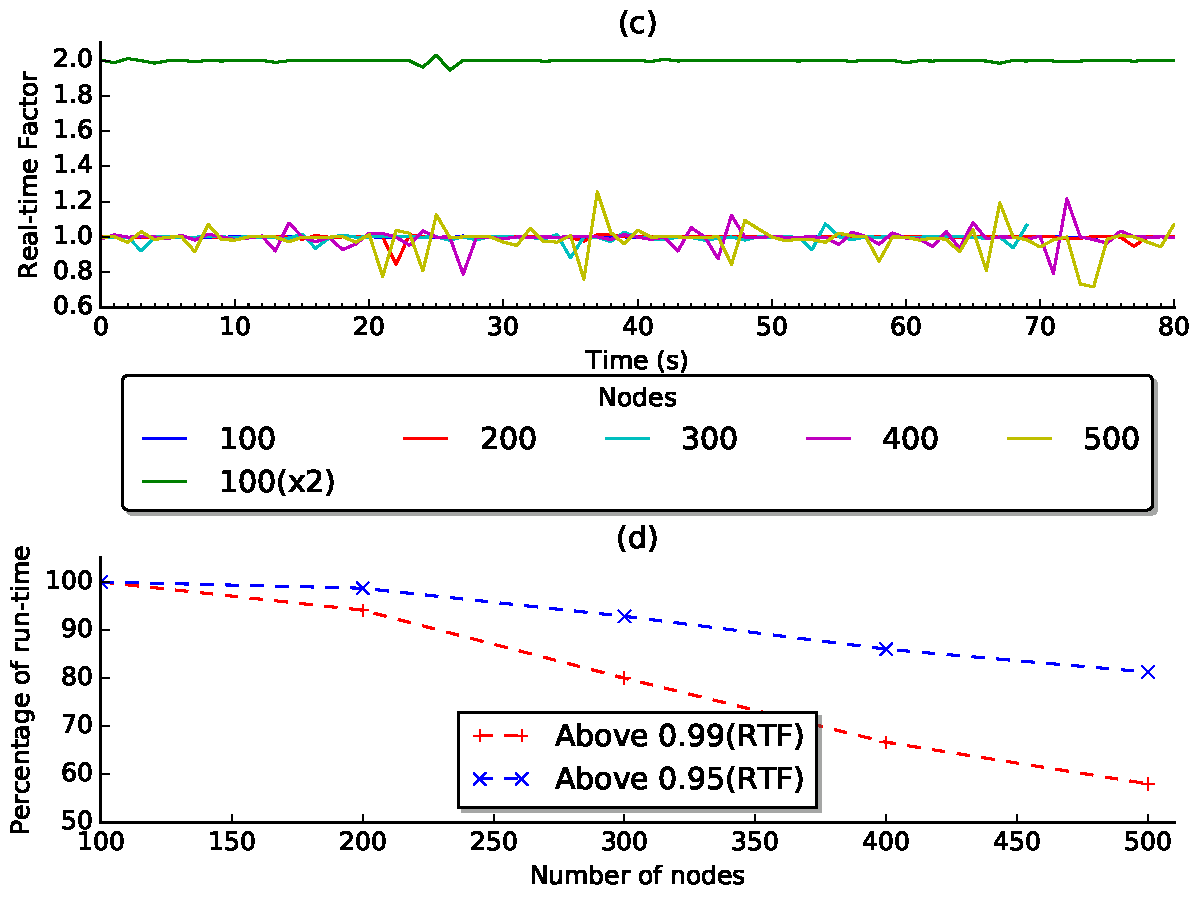
\includegraphics[width=0.5\textwidth]{plots/plot2.pdf}
  \caption{Figure (a) shows how the simulator speed fluctuates over time. Figure (b) shows the percentage of the total run time which the simulation maintains above 99\% and 95\% of its target speed.}
  \label{fig:simulator_scalability}
\end{figure}

Extending further, we also performed tests on running Ard\'{a}n at faster than real-time, at 200\% speed. In this mode, the game engine and its physics engine match the speed of the simulator, resulting in all activity increasing in speed, as opposed to simply increasing the walking speed of individuals. The results in figure \ref{fig:simulator_scalability} show that roughly half the number of nodes can be simulated in time with the game engine, with little fluctuation.

\subsection{Faster-than-real-time Performance} % (fold)
\label{sub:faster_than_real_time_performance}

% subsection faster_than_real_time_performance (end)

% \section{Requirements}
% \label{sec:Requirements}
% Define the list of key requirements described in workshop paper.

% \section{Framework} % (fold)
% \label{sec:framework}

% \subsection{CPS Simulation} % (fold)
% \label{sub:cps_simulation}

% \subsection{Virtual World Simulation} % (fold)
% \label{sub:virtual_world_simulation}
% % subsection virtual_world_simulation (end)
% % subsection cps_simulation (end)

% \subsection{Communication Model} % (fold)
% \label{sub:communication_model}
% % subsection communication_model (end)

% \subsection{Time} % (fold)
% \label{sub:time}
% % subsection time (end)
% % section framework (end)

% \section{Co-simulation} % (fold)
% \label{sec:co_simulation}

% \subsection{Performance} % (fold)
% \label{sub:performance}

% \subsection{Discussion} % (fold)
% \label{sub:discussion}

% subsection discussion (end)
% subsection performance (end)
% section co_simulation (end)

% \section{Features}
% Ard\'{a}n\footnote{Ard\'{a}n, pronounced ``awrd-awn'', is the Gaelic word for platform.} combines a high-performance 3D game engine, Unreal Engine 4, with an existing multi-level sensor network simulator, Cooja, to provide an end to end solution for testing real sensor network applications in virtual world environments. The rest of this section describes the novel key features and high-level design of Ard\'{a}n.

% Ard\'{a}n provides developers with a rich tool-set to control and observe the simulation environment, including 3D design and placement, time-control, phenomena-on-demand and visualisation.

% \subsection{3D design and placement}
% \label{sub:3D design and placement}
% A key part of many sensor network projects is understanding how many and where to place devices within the environment to achieve some desired objective, such as coverage, reliability or detection accuracy. Using Ard\'{a}n developers are able to easily scale up or down the size of the network and move devices around the environment to test different configurations.

% \subsection{Time Control}
% \label{sub:Time Control}
% Unlike in real world deployments, developers have the power to control time in the simulated world. Developers can: stop-the-clock, freezing both the simulation and world in time, whilst giving them full control over what they see, allowing more time to observe the environment and move between points of interest; slow down time, giving developers more time to observe or control the simulation; or even speed up time, providing desired results in considerably less time.

% \subsection{Phenomena-on-demand}
% \label{sub:Phenomena-on-demand}
% In order to fully test sensor network applications in the real-world, developers often need to wait for or even force desired phenomena to occur and then observe how their system reacts. However, exercising control over the real-world can be a difficult and time-consuming challenge, and sometimes not possible (e.g., fire), due to health and safety concerns.

% Using Ard\'{a}n, developers can take direct control of a virtual person or script intelligent virtual crowds to carry out tasks, such as walking between points, avoidance, following or interacting with objects. Figure \ref{fig:views} shows people walking up and down a corridor, avoiding each other's path. Unlike using trace data, genuine or created, developers can easily tweak scenarios, such as moving sensors, people or adjusting behaviour, to test subtle or significant variations. Developers can also create scenarios that are difficult or dangerous to reproduce in the real world, such as emergency situations, and repeatedly test their applications without risk.

% \subsection{Visualisation}
% \label{sub:Visualisation}
% Ard\'{a}n provides developers tools to overlay visualisations of network and sensor meta-information on top of the virtual world to help understand how the network is running, allowing developers to see information such as how network paths form as packets are sent, as well as transmissions, receptions, interruptions. In figure \ref{fig:views}, sending devices are highlighted with a circle and receiving devices are connected by an arrow to the sender, each device is represented with its own colour, to help differentiate simultaneous transmissions.

% \subsection{Virtual Sensors and Actuators}
% \label{sub:Virtual Sensors and Actuators}
% Within Ard\'{a}n we have modeled several basic sensors and actuators, including motion detectors, buttons, lights and location. These act as virtual hardware for the simulated sensors, allowing the simulation to interact with the virtual world. Virtual sensors can be designed to model a real sensors behaviour, or be virtually improved, providing higher accuracy or more features, not possible with existing hardware.




\section{Summary} % (fold)
\label{sec:summary}

% section summary (end)


% \section{Design Goals}
% \label{sec:Design Goals / Requirements}

% \subsection{Exploit 3D game engine to simulate CPS environment}
% \label{sub:Virtual Environments}
% Exploiting the use of 3D game engines simulate CPS in a virtual environment.

% \subsection{Analysing CPS in a 3D virtual world}
% \label{sub:analysing_cps_in_a_3d_virtual_world}
% Developing new tools to view and analyse CPS in 3D virtual environments.

% \subsection{Analysing CPS in the real world using AR} % (fold)
% \label{sub:analysing_cps_in_the_real_world_using_ar}
% How can we use techniques developed from previous chapter and apply them to analysing real-world CPS using AR technology.

% subsection analysing_cps_in_the_real_world_using_ar (end)
% \subsection{Comparing and learning from Virtual vs Real-world executions}
% \label{sub:Trained environment Models}
% Exposing the run-time differences of different network runs, to discover insights, highlight issues or debug new code.
% Building more accurate and scenario specific environment models by cross-training using pre-deployment data, creating more accurate localised models on environmental data, such as people movement/interaction, device models, temperature, operation speed etc.

% \subsection{Formally specifiying rules and testing counterexamples}
% \label{sub:formal}